
	\subsection{Polynomial-Time Reductions}
	A reduction $Q \leadsto R$ from a problem $Q$ to another problem $R$ represents $Q$ as a case of $R$, which we already know how to solve. Examples of reductions that we have seen are,
	\begin{align*}
		&\text{Bipartite Matching $\leadsto$ Maximum Flow} \\
		&\text{Bipartite Vertex Cover $\leadsto$ Minimum Cut} \\
		&\text{Maximum Flow $\leadsto$ Linear Programming}
	\end{align*}

	\begin{defn}[Karp Reductions]
		A \textbf{Karp reduction} $Q \leadsto R$ from $Q$ to $R$ is an algorithm that produces an instance \texttt{I'} of $R$ given an instance $\texttt{I}$ of $R$. The algorithm runs in polynomial time in the size of \texttt{I} and \texttt{I'} is a \texttt{YES} instance of $R$ if and only if $\texttt{I}$ is a \texttt{YES} instance of $Q$\footnote{We write $Q \leq_p R$, which can be read as "$Q$ is polynomial-time reducible to $R$" or "$R$ is at least as hard as $Q$."}.
	\end{defn}

	\begin{rmk}
		Let $Q \leadsto R$. 
		\begin{itemize}
			\item If $R$ is easy to solve, then $Q$ is easy to solve
			\[R_{\texttt{easy}} \implies Q_{\texttt{easy}}\]
			\item If $Q$ is hard to solve, then $R$ is hard to solve
			\[Q_{\texttt{hard}} \implies R_{\texttt{hard}}\]
			\item If $Q$ is easy to solve, then this tells us nothing about $R$ 
			\[Q_{\texttt{hard}} \implies \text{Nothing}\]
		\end{itemize}
	\end{rmk}

	\begin{defn}[Vertex Cover Problem]
		We are given a graph $G = (V, E)$ and an integer $c$. We want to know if $G$ contains a set of at most $c$ vertices that are incident to each edge.
	\end{defn}

	\begin{defn}[Independent Set Problem]
		We are given a graph $G = (V, E)$ and an integer $k$. We want to know if $G$ contains a set of at least $k$ vertices that are mutually non-adjacent.
	\end{defn}

	\begin{ex}{Independent Set $\leadsto$ Vertex Cover}{label}
		If $S \subseteq V$ is an independent set, then $V - S$ is a vertex cover. A polynomial time algorithm for \textbf{Vertex Cover} can be used to give a polynomial time algorithm for \textbf{Independent Set}.
		\begin{align*}
			\text{There is an independent set of size at least $k$}
		\end{align*}
		\[\iff\]
		\begin{align*}
			\text{There is a vertex cover of size at most $n-k$}
		\end{align*}
		\noindent Similarly, Vertex Cover $\leadsto$ Independent Set.
	\end{ex}

	\begin{defn}[Set Cover Problem]
		We are given sets $S_1, S_2, \cdots, S_n \subseteq W$ and an integer $k$. We want to know if there is a collection of at most $k$ sets that cover every element of $W$.
	\end{defn}

	\begin{ex}{Vertex Cover $\leadsto$ Set Cover}{label}
		Suppose that we are given a graph $G = (V, E)$. Define,
		\[S_v := \{e \text{ $|$ $v$ is an endpoint of $e$}\}\]
		\noindent for each $v \in V$. Set $W = \{e \text{ $|$ } e \in E\}$. Then a set cover of size $k$ corresponds to a vertex cover of size $k$, and a polynomial time algorithm for \textbf{Set Cover} can be used to give a polynomial time algorithm for \textbf{Vertex Cover}.
	\end{ex}

	\begin{defn}[Satisfiability Problem]
		Suppose that we have,
		\begin{itemize}
			\item Boolean variables $x_1, \cdots, x_n$
			\item Clauses $C_1, \cdots, C_m$ which are disjunctions of literals,
			\[C_{j}=x_{2} \lor \bar{x}_{5} \lor \bar{x}_{6} \lor x_{8} \lor \bar{x}_{9}\]
			\item Literals $x_i$ and $\bar{x_i} \in \{\texttt{True}, \texttt{False}\}$ for each variable $x_i$
		\end{itemize}
		\noindent We want to know if there is an assignment that satisfies every clause.
	\end{defn}

	\begin{defn}[3-Satisfiability]
		\textbf{3-satisfiability} is a special case of the satisfiability problem, where every clause has exactly three literals.
		\[\text{e.g., }\quad \left(x_{1} \lor \bar{x}_{2} \lor x_{5}\right) \wedge\left(x_{2} \lor \bar{x}_{3} \lor \bar{x}_{4}\right) \wedge\left(\bar{x}_{1} \lor x_{3} \lor x_{4}\right) \wedge\left(\bar{x}_{3} \lor \bar{x}_{4} \lor \bar{x}_{5}\right)\]
	\end{defn}

	\begin{ex}{SAT $\leadsto$ 3-SAT}{label}
		Clearly SAT $\leadsto$ 3-SAT. We can also show that SAT $\leadsto$ 3-SAT. 
		
		\begin{rmk}
		A variable assignment satisfies $\ell_1 \lor \ell_2 \lor \cdots \lor \ell_k$ if and only if the same variable assignment satisfies,
		\[\left(\ell_{1} \lor \cdots \lor \ell_{p} \lor y\right) \wedge\left(\bar{y} \lor \ell_{p+1} \lor \cdots \lor \ell_{k}\right)\]
		\noindent for some \texttt{True} / \texttt{False} assignment of $y$.
		\label{satisfiability}
	\end{rmk}

		\begin{itemize}
			\item We need to convert an instance \texttt{I} of SAT into an instance \texttt{I'} of 3-SAT. To do this, take each clause $C$ in \texttt{I} and mimic it via a set of clauses of size 3 with additional variables
			\item Take a clause $C = \ell_{1} \lor \ell_{2} \lor \cdots \ell_{k}$. There are three cases,
			\begin{itemize}
				\item If $k = 2$, we can pick $y$ and $\bar{y}$ as follows:
				
				\resizebox{.6\hsize}{!}{
				$\ell_{1} \lor \ell_{2} \quad \Longrightarrow \quad\left(\ell_{1} \lor \ell_{2} \lor y\right) \wedge\left(\ell_{1} \lor \ell_{2} \lor \bar{y}\right)$}

				\item If $k = 1$, we can pick $y_1, y_2$ and $\bar{y_1}, \bar{y_2}$ as follows:
				
				\resizebox{.9\hsize}{!}{
				$\ell_{1} \implies \left(\ell_{1} \lor y_{1} \lor y_{2}\right) \wedge\left(\ell_{1} \lor y_{1} \lor \bar{y}_{2}\right) \wedge\left(\ell_{1} \lor \bar{y}_{1} \lor y_{2}\right) \wedge\left(\ell_{1} \lor \bar{y}_{1} \lor \bar{y}_{2}\right)$}

				\item If $k \geq 3$, we apply Remark \ref{satisfiability} recursively.
			\end{itemize}
		\end{itemize}.
		Thus, for $C = \ell_{1} \lor \ell_{2} \lor \cdots \ell_{k}$, we have:
		\begin{itemize}
			\item $k - 2$ clauses in \texttt{I'}
			\item $k - 3$ new variables in \texttt{I'}
		\end{itemize}
		so a polynomial time algorithm for \textbf{3-SAT} can be used to give a polynomial time algorithm for \textbf{SAT}.
	\end{ex}

	\begin{ex}{3-SAT $\leadsto$ Independent Set}{label}
		\begin{itemize}
			\item We need to convert an instance \texttt{I} of 3-SAT,
			\[C=x_{1} \vee \bar{x}_{2} \vee x_{5}\]
			\noindent into an instance \texttt{G} of Independent Set. For each clause $C$ in \texttt{I}, we have a triangle in \texttt{G},

			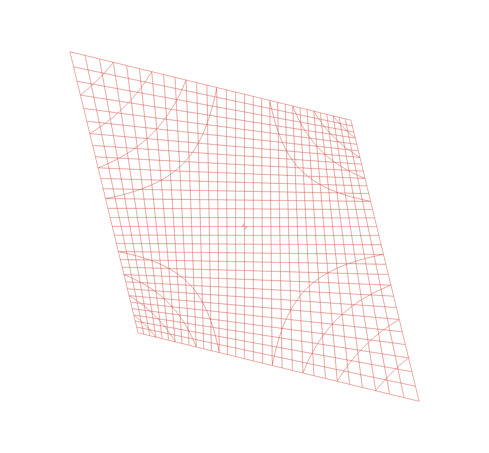
\includegraphics[width=\textwidth]{fig-12.png}

			\item We add an edge between each copy of $x_i$ and $\bar{x_i}$,

			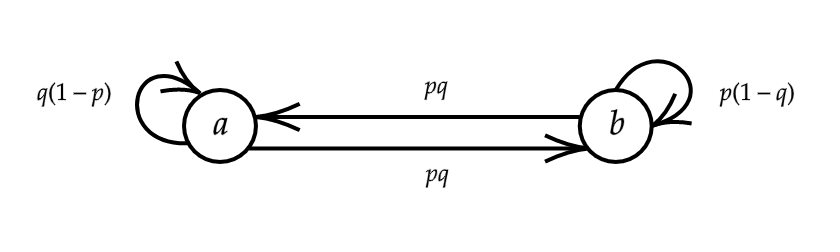
\includegraphics[width=\textwidth]{fig-13.png}
		\end{itemize}
		There is a satisfying assignment for \texttt{I} if and only if there is an independent set in $G$ whose size is equal to the number of clauses. To see this, note that,
		\begin{itemize}
			\item There are $m$ triangles in $G$ and an independent set $S$ uses at most one vertex per triangle. This means that,
			\[|S| \leq m\]
			\item If $S$ selects $x_i$, then $x_i$ is set to \texttt{True}. We cannot also select a vertex for $x_i$, so $S$ induces a valid assignment
			\item If $S$ selects $x_i \in C_j$, then $C_j$ is satisfied
			\item Thus, an independent set of size $m$ in $G$ gives a satisfying assignment for \texttt{I} and any satisfying assignment for \texttt{I} induces an independent set of size $m$ in $G$ 
		\end{itemize}
 	\end{ex}

 	\subsection{NP Completeness}
 	\begin{marginfigure}
 		Equivalently, $NP$ is,
 		\begin{itemize}
 			\item The set of decision problems whose \texttt{YES} instances can be verified in polynomial time
 			\item The set of decision problems that can be solved in exponential time by Brute-Force Search
 		\end{itemize}
 		\noindent These definitions are equivalent because any \texttt{YES} instance has a certificate of size $poly(n)$, and there are an exponential, i.e., $2^{poly(n)}$ number of such certificates.
 	\end{marginfigure}

 	\begin{defn}[P]
 		The class \textbf{P} is the set of decision problems which can be solved in polynomial time by a deterministic computer.
 	\end{defn}

 	\begin{defn}[NP]
 		The class \textbf{NP} is the set of decision problems which can always be solved in polynomial time by a non-deterministic computer.
 	\end{defn}

 	\begin{rmk}[$P \neq NP$]
 		The \textbf{conjecture} that $P \neq NP$ states that computation is harder than verification. We know that $P \subseteq NP$ since we can compute and verify a solution to a problem $R \in P$ in polynomial time.
 	\end{rmk}

 	\begin{defn}[NP Complete]
 		A problem $R$ is \textbf{NP Complete} if for every $Q \in NP$, there is a polynomial time reduction\footnote{The reduction maps \texttt{YES} instances of $Q$ into \texttt{YES} instances of $R$, and it maps \texttt{NO} instances of $Q$ into \texttt{NO} instances of $R$} from $Q$ to $R$.
 	\end{defn}

 	 \begin{defn}[coNP]
 	 	 The class \textbf{coNP} is the set of decision problems whose \texttt{NO} instances can be verified in polynomial time.
 	\end{defn}

 	\begin{defn}[coNP Complete]
 		A problem $R$ is \textbf{coNP Complete} if for every $Q \in coNP$, there is a polynomial time reduction from $Q$ to $R$.
 	\end{defn}

 	\begin{defn}[Good Characterization]
 		A problem $R \in NP \cap coNP$ has a \textbf{good characterization} if has a polynomial \texttt{YES} and \texttt{NO} certificate.  
 	\end{defn}

 	\begin{ex}{Good Characterizations}{label}
 		The following problems have a good characterization,

 		\vphantom{.}

 		\resizebox{\textwidth}{!}{
 		\begin{tabular}{lll}
 		\textbf{Problem} & \textbf{\texttt{YES} Instance} & \textbf{\texttt{NO} Instance} \\ \hline
 		Maximum Flow & Flow & Minimum Cut \\
 		Bipartite Matching & Matching & Vertex Cover \\
 		Linear Programming & Feasible Primal & Feasible Dual \\
		\end{tabular}}
 	\end{ex}

 	\begin{rmk}
 		The complement of an NP Complete problem is in coNP.
 	\end{rmk}

 	\begin{rmk}
 		$P = NP \implies NP = coNP$
 	\end{rmk}

 	\begin{proof}
 		Problems in $P$ have a \texttt{YES} and \texttt{NO} certificate. If $P = NP$ then every problem in $NP$ has a short \texttt{YES} and \texttt{NO}. This implies,
 		\[P \subseteq coNP\]
 		\noindent Any problem $R \in coNP$ has $R^c \in NP = P \implies R \in P = NP$.
 	\end{proof}

 	\begin{ex}{Cliques}{label}
 		The problem of determining if a set $S$ of vertices is a clique is in NP. We can check if the vertices are pairwise adjacent, which is polynomial in the size of $S$.
 	\end{ex}

 	\begin{marginfigure}
 		\begin{center}
 						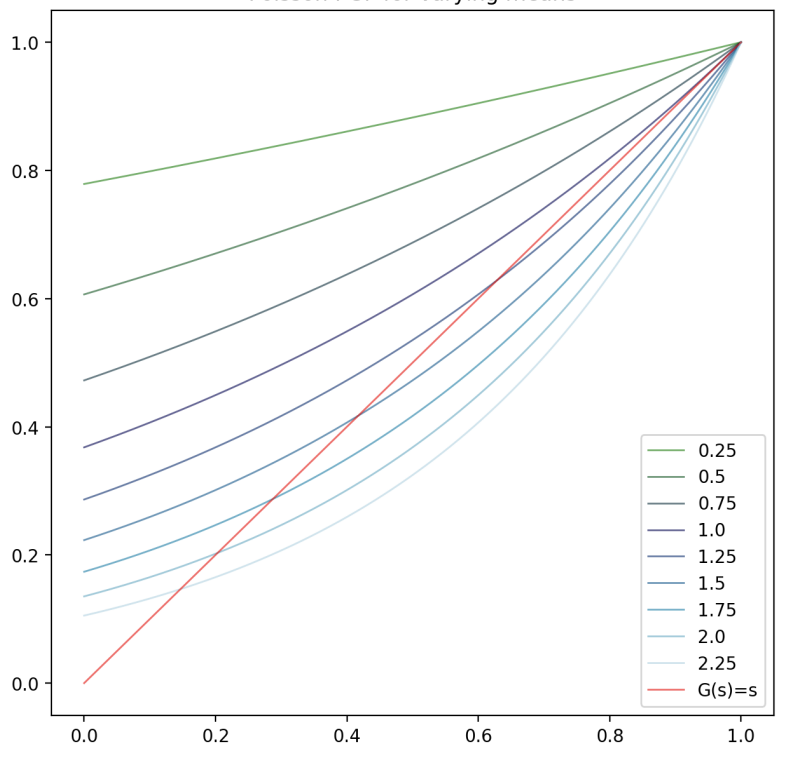
\includegraphics[width=\textwidth]{fig-16.png}
 			\end{center}
 	\end{marginfigure}

 	\begin{defn}[Cook's Theorem]
 		Satisfiability is NP Complete.
 	\end{defn}

 	\begin{marginfigure}
 		$3-SAT$, Independent Set, Vertex Cover, and Set Cover are NP Complete.
 	\end{marginfigure}

 	\begin{rmk}[Proving NP Completeness]
 		Do the following,
 		\begin{enumerate}
 			\item For your new problem $R$, show that $R \in NP$
 			\item Find an $NP$-complete problem $Q$ such that $Q \leadsto R$
 		\end{enumerate}
 	\end{rmk}

 	\begin{defn}[Graph-Coloring Problem]
 		A \textbf{vertex coloring} of a graph $G = (V,E)$ is an assignment of colors to vertices such that adjacent vertices recieve different colors. The chromatic number $\chi(G)$ is the minimum number of colors required for a valid coloring to exist. We want to know if there exists a 3-coloring of $G$.
 	\end{defn}

 	\begin{ex}{3-SAT $\leadsto$ 3-Coloring}{label}
 		First, we can show that 3-coloring is in NP by checking,
 		\begin{itemize}
 			\item $\leq 3$ colors are used
 			\item Every vertex recieves a color $c$
 			\item $c(u) \neq c(v)$ for all $(u,v) \in E$
 		\end{itemize}
 		
 		Second, we reduce from $3-SAT$ to 3-Coloring:
 		\begin{itemize}
 			\item We need to convert an instance \texttt{I} of 3-SAT into an instance \texttt{I'} of 3-Coloring. To do this, we build a graph $G$ as follows,
 			\begin{itemize}
 				\item There is a vertex for each literal $x_1, \bar{x_1}, x_2, \cdots, x_n, \bar{x_n}$
 				\item There are three vertices, $T, F, B$
 				\item The vertices are connected as follows,
 					\begin{center}
 						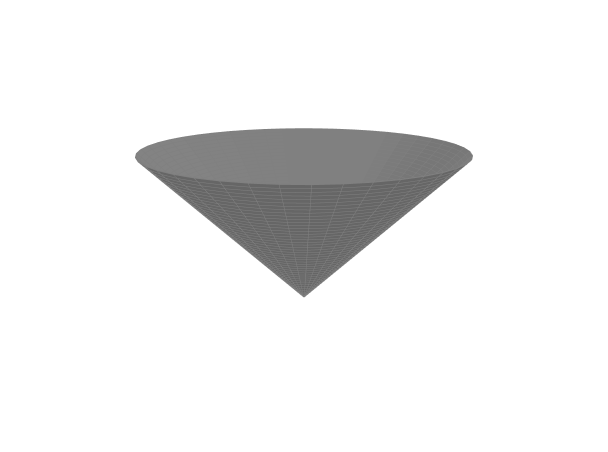
\includegraphics[width=0.5\textwidth]{fig-14.png}
 					\end{center}
 			\end{itemize}
 			\item Define the following,
 				\begin{itemize}
 					\item $\texttt{Green} = \texttt{True}$
 					\item $\texttt{Red} = \texttt{False}$
 					\item $\texttt{White} = \texttt{BLANK}$
 				\end{itemize}
 			\noindent so that the colors of $x_1, \bar{x_1}, x_2, \cdots, x_n, \bar{x_n}$ give a valid \texttt{True} and \texttt{False} assignment of variables.
 			
 			\item Design a gadget for each clause which can be 3-colored if and only if the clause is satisfied. Each gadget clause contains 6 new vertices which we connect to the assignment
 			 \begin{center}
 						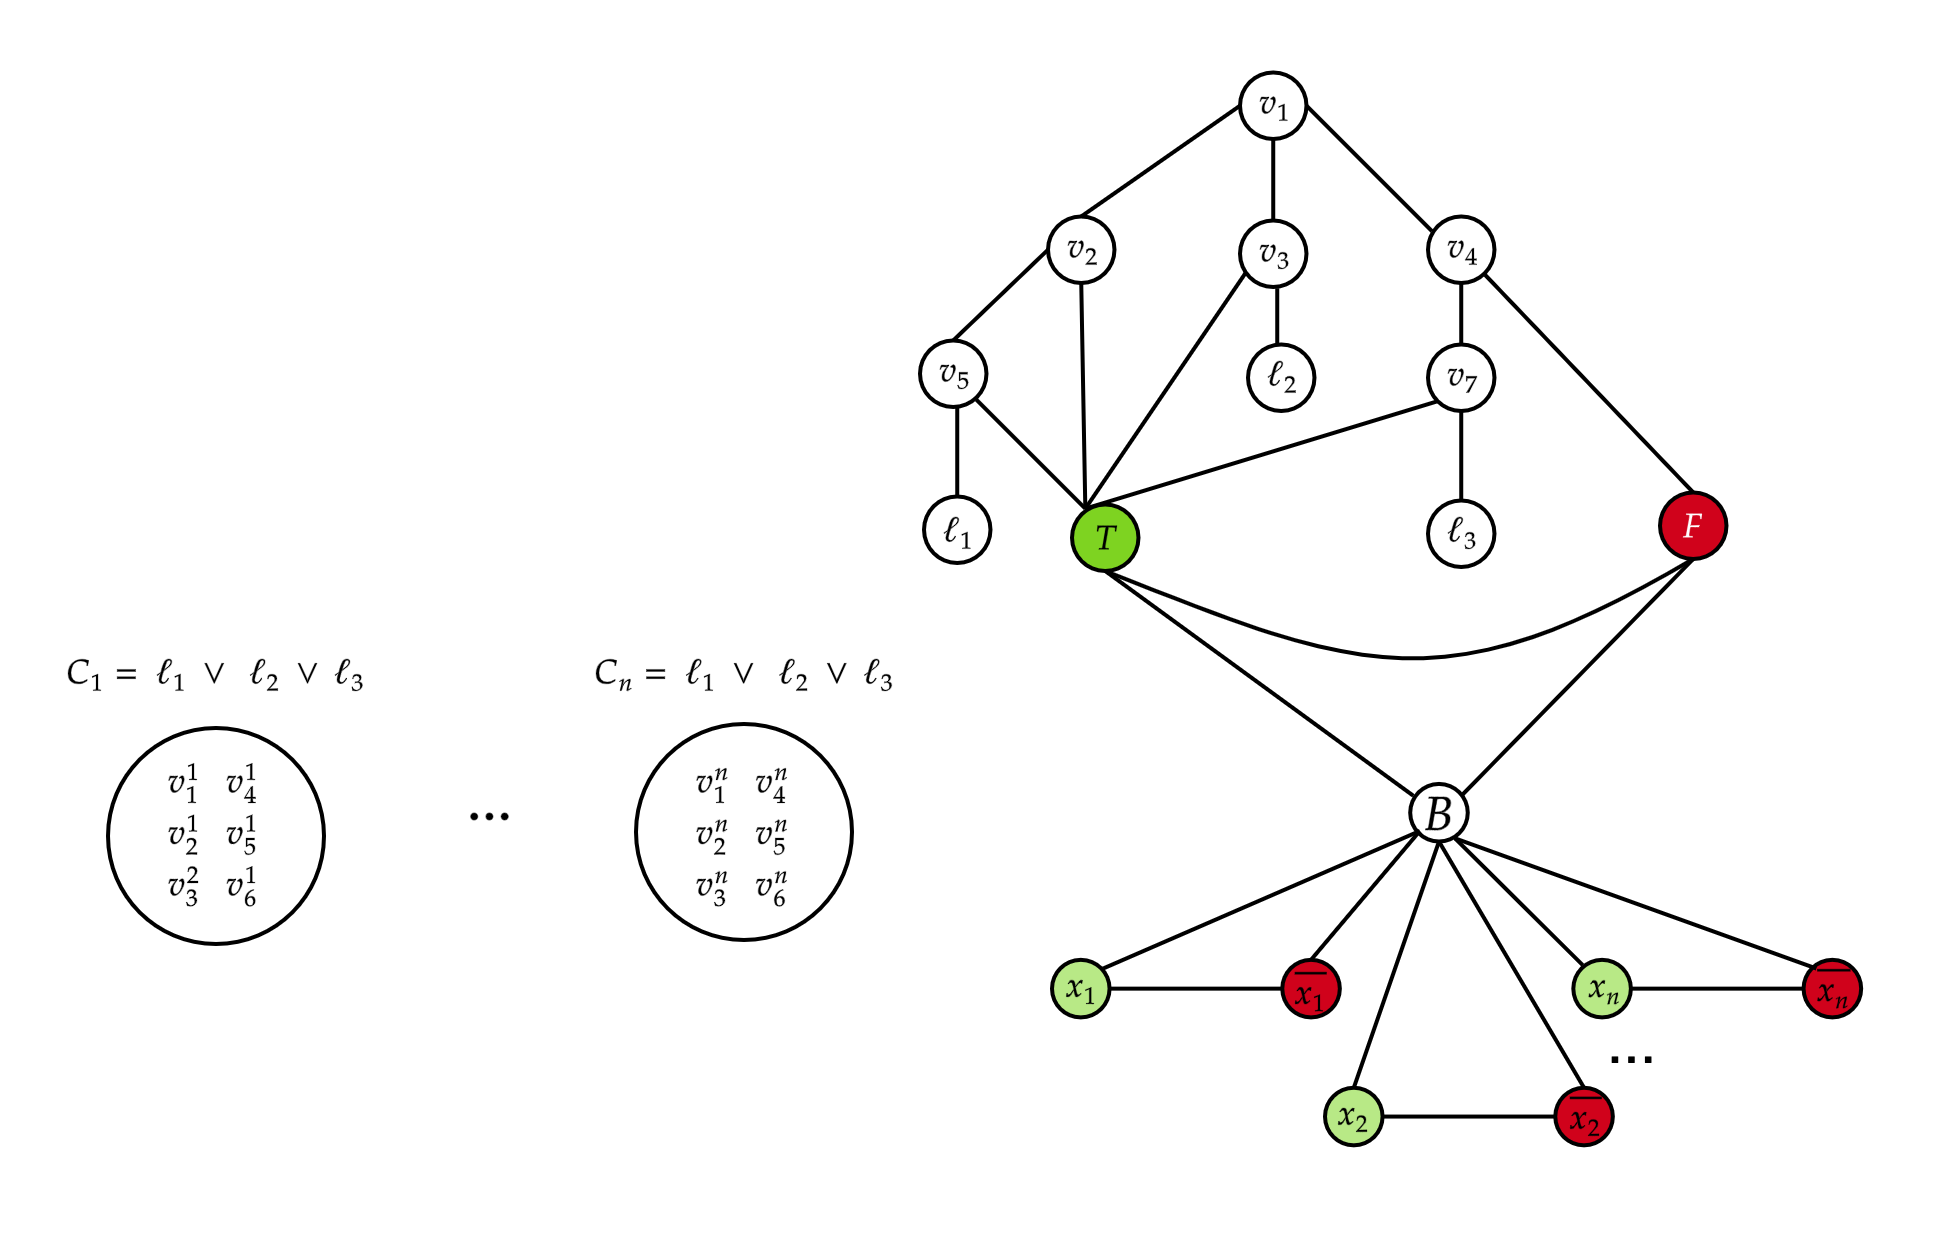
\includegraphics[width=\textwidth]{fig-18.png}
 			\end{center}

 			\item The clause for $C$ is $\ell_1 \lor \ell_2 \lor \ell_3$. We can check coloring for,
 			\begin{align*}
 				&\text{Case 1. $(\ell_1 = F, \ell_2 = F, \ell_3 = T)$} \\
 				&\text{Case 2. $(\ell_1 = F, \ell_2 = T, \ell_3 = F)$} \\
 				&\cdots \\
 				&\text{Case 8. $(\ell_1 = F, \ell_2 = F, \ell_3 = F)$}
 			\end{align*}
 			\item We discover that Case 8 cannot be colored validly, so $G$ can be 3-coloured if and only if $\texttt{I}$ is satisfiable. This completes the polynomial reduction 3-SAT $\leadsto$ 3-Colouring
 		\end{itemize}
 	\end{ex}

 	\begin{defn}[Prime Factorization Problem]
 		Given integers $N$ and $k$, we want to determine if $N$ has a prime factor $\leq k$.
 	\end{defn}

 	\begin{marginfigure}
 		The \texttt{YES} instance for prime factorization works because even if $p$ is not prime, it has some prime factorization.
 	\end{marginfigure}

 	\begin{ex}{Prime Factorization}{label}
 		We believe that prime factorization is in $NP \cap coNP - P$.
 		\begin{itemize}
 			\item Prime factorization is in NP
 			\begin{itemize}
 				\item (\texttt{YES} Instance) Give an integer $p \leq k$ such that $p |N$. 
 			\end{itemize}
 			\item Prime factorization is in coNP
 			\begin{itemize}
 				\item (\texttt{NO} Instance) Given the unique prime factorization $N = p_1p_2 \cdots p_n$, we verify that each $p_i > k$ and confirm that $p_i$ is prime in polynomial time
 			\end{itemize}
 		\end{itemize}
 	\end{ex}

 	\begin{marginfigure}
 		\textbf{Well-Known NP Complete Problems:}
 		\begin{itemize}
 			\item (Hamiltonial Cycle Problem) Given $G = (V, E)$, we want to determine if $G$ contains a cycle that uses every vertex exactly once
 			\item (Hamiltonian Path Problem) Given $G = (V, E)$, we want to determine if $G$ contains a path that uses every vertex exactly once
 			\item (Partition Problem) Given integers $x_1, \cdots, x_n \geq 0$, we want to determine if $\exists$ a subset $S \subseteq [n]$ s.t.,
 			\[\sum_{i \in S} x_i = \sum_{i \not\in S} x_i\]
 			\item (Maximum Cut Problem) Given $G = (V, E)$ and an integer $k$, we want to determine if $G$ contains a cut $\delta(S)$  containing at least $k$ edges
 		\end{itemize}
 	\end{marginfigure}

 	\begin{ex}{Taxonomy of Easy and Hard Problems}{label}
 		\resizebox{\textwidth}{!}{
 		\begin{tabular}{ll}
 		\textbf{Easy Problems}		 & \textbf{Hard Problems}	      \\ \hline
		Minimum Cut                & Maximum Cut                  \\ 
		Euler Circuit              & Hamiltonian Cycle            \\ 
		2-SAT                      & 3-SAT                        \\ 
		2-Coloring                 & 3-Coloring                   \\ 
		Shortest Path              & Longest Path                 \\ 
		Shortest Even $(s-t)$ Path & Shortest Even $(s-t)$ Dipath \\ 
		Linear Programming         & Integer Programming          \\ 
		\end{tabular}}
 	\end{ex}

 	\begin{ex}{Taxonomy of Hard Problems}{label}
 		\begin{tabular}{ll}
 		\textbf{Group} & \textbf{Example} \\ \hline
 		Packing Problems
 				& \tabitem Independent Set \\
 				& \tabitem Clique \\
 				& \tabitem Set Packing \\ \hline
			
 		Covering Problems
 				& \tabitem Vertex Cover \\
 				& \tabitem Set Cover \\ \hline

 		Partitioning Problems
 				& \tabitem 3-Coloring \\
 				& \tabitem 3D-Matching \\
 				& \tabitem Maximum Cut \\ \hline

 		Sequencing Problems
 				& \tabitem Hamiltonian Path \\
 				& \tabitem Travelling Salesman \\ \hline

 		Numerical Problems
 				& \tabitem Partition \\
 				& \tabitem Knapsack \\ \hline
		\end{tabular}
 	\end{ex}

 	\begin{ex}{Integer Programming}{label}
 		We are given an integer problem and an integer $k$. We want to determine if there is a feasible solution with value at least $k$. The minimization case is analogous. 
 	\end{ex}

 	\subsection{PSpace and Complexity Classes}
 	\begin{defn}[Exp]
 		The class \textbf{Exp} is the set of decision problems that can be solved in exponential time by a deterministic computer.
 	\end{defn}

 	\begin{defn}[NExp]
 		The class \textbf{NExp} is the set of decision problems that can be solved in exponential time by a non-deterministic computer\footnote{
 		Equivalently, this is the set of decision problems whose \texttt{YES} instances can be verified in exponential time.}.
 	\end{defn}

 	\begin{defn}[PSpace]
 		The class \textbf{PSpace} is the set of decision problems that can be solved by an algorithm using polynomial space\footnote{$P \subseteq PSpace$ since a problem that requires polynomial time uses a polynomial amount of space.}.
 	\end{defn}

 	\begin{defn}[PSpace Complete]
 		A problem $R$ is \textbf{PSpace Complete} if for every $Q \in PSpace$, there is a polynomial space reduction from $Q$ to $R$.
 	\end{defn}

 	 \begin{defn}[ExpSpace]
 		The class \textbf{ExpSpace} is the set of decision problems that can be solved by an algorithm using exponential space.
 	\end{defn}

 	\begin{thm}
 		NP $\subseteq$ PSpace.
 	\end{thm}

 	\begin{proof}
 		\noindent It suffices to show that 3-SAT $\in$ PSpace since there exists a polynomial reduction for any problem $Q \in NP$ such that $Q \leadsto$ 3-SAT. This reduction necessarily uses a polynomial amount of space. Take an instance \texttt{I} of 3-SAT. Let each binary string $b_1b_2 \cdots b_n$ of length $n$ encode a \texttt{True}/\texttt{False} assignment of the variables.
 		\[b_i = \begin{cases}
 			1 & x_i = \texttt{True} \\
 			0 & \bar{x_i} = \texttt{True}
 		\end{cases}\]

 		\begin{algorithm}
	  \caption{3SAT $\in$ PSpace}\label{3Sat}
	  \Comment{Initialize $b$ to be the $0$ vector.}
	  \Function{3SAT($b, \texttt{I}$)}{
	    \ForEach{$b \in C(\texttt{I})$}{
		    	\If{$b \text{ does not satisfy \texttt{I}}$}{
		    	\Comment{Increase $b_n$ by $1$.}
		    		$b \assign b + 1$\;
		      }
		    	\Else{
		    	  \Return{$b$}\;}
		     	}
	     	}
	\label{3satalgo}
	\end{algorithm}

 	\noindent Algorithm \ref{3satalgo} either finds a satisfying assignment, or it confirms that $\texttt{I}$ is not satisfiable. It runs in exponential time by counting to $2^n$, but it only uses a polynomial amount of space.
 	\end{proof}

 	\begin{rmk}
 		If $Q \in$ PSpace, then $Q^c \in$ PSpace. Thus, $coNP \subseteq$ PSpace.
 	\end{rmk}

 	\begin{rmk}
		It has been conjectured that,
		\[\mathbf{P} \subseteq \mathbf{N P} \subseteq \mathbf{P S P A C E} \subseteq \mathbf{E X P} \subseteq \mathbf{N E X P} \subseteq \mathbf{E X P S P A C E}\]
	\end{rmk}

 	\begin{defn}[Q-Satisfiability]
		\textbf{Q-satisfiability} is a special case of the satisfiability problem, where every clause alternates between $\forall$ and $\exists$.
		\[\text{e.g., }\exists x_{1} \forall x_{2} \exists x_{3} \forall x_{4} \cdots \quad C_{1} \wedge C_{2} \wedge \cdots \wedge C_{m}\]
	\end{defn}

	\begin{marginfigure}
		The mix of universal and existential quantifiers arises commonly in games,
		\begin{align*}
			&\exists \text{ a move such that,} \\
			&\forall \text{ moves by the opponent,} \\
			&\text{etc}.
		\end{align*}
	\end{marginfigure}

	\begin{ex}{QSat $\in$ PSpace}{label}
		Let $\phi(x_1, x_2, \cdots, x_n) = C_1 \land C_2 \land \cdots C_m$ and consider,
		\[\exists x_{1} \forall x_{2} \exists x_{3} \forall x_{4} \cdots \Phi\left(x_{1}, x_{2}, \ldots, x_{n}\right)\]

		We want to solve the assignment recursively. At step $i$,
		\[x_1 = \ell_1, \quad x_2 = \ell_2  \quad \cdots \quad x_{i-1} = \ell_{i-1}\]

		\textbf{Case 1.} $i$ is odd.
		$x_i$ is associated with $\exists$. We want,
		\[\Phi\left(\ell_{1}, \ldots, \ell_{i-1}, x_{i}, x_{i+1}, \ldots, x_{n}\right)=1\]
		for $\ell_{1}, \ldots, \ell_{i-1}$ fixed. This is true if and only if,
		\[\Phi\left(\ell_{1}, \ldots, \ell_{i-1}, 0, x_{i+1}, \ldots, x_{n}\right)=1\]
		\[\text{or}\]
		\[\Phi\left(\ell_{1}, \ldots, \ell_{i-1}, 1, x_{i+1}, \ldots, x_{n}\right)=1\]

		\textbf{Case 2.} $i$ is even.
		$x_i$ is associated with $\forall$. We want,
		\[\Phi\left(\ell_{1}, \ldots, \ell_{i-1}, x_{i}, x_{i+1}, \ldots, x_{n}\right)=1\]
		for $\ell_{1}, \ldots, \ell_{i-1}$ fixed. This is true if and only if,
		\[\Phi\left(\ell_{1}, \ldots, \ell_{i-1}, 0, x_{i+1}, \ldots, x_{n}\right)=1\]
		\[\text{and}\]
		\[\Phi\left(\ell_{1}, \ldots, \ell_{i-1}, 1, x_{i+1}, \ldots, x_{n}\right)=1\]


		\textbf{Time Complexity:}

		To solve $\phi(x_1, x_2, \cdots, x_n)$, we solve 2 subproblems,
		\[T(n) \leq 2 \cdot \underbrace{T(n-1)}_{\text{$x_n$ is fixed}} + \text{poly}(n,m)\]
		for $n$ variables and $m$ clauses.

		\vphantom{.}

		\textbf{Space Complexity:}

		We can re-use space for each subproblem.
		\begin{itemize}
			\item Solve the case $x_1 = 0$
			\item Save the solution $\phi(0, x_2, \cdots, x_n) = 0$ or $\phi(0, x_2, \cdots, x_n) = 1$
			\item Delete all other memory and reuse the space to solve $x_1 = 1$
		\end{itemize}
		This gives the space complexity,
		\[S(n) \leq S(n-1) + \text{poly}(n,m)\]
	\end{ex}

	\begin{defn}[2Exp]
		The class \textbf{2Exp} is the set of decision problems that can be solved in double exponential time, $2^{2^{\text{poly}(n)}}$ by a deterministic computer. Similar definitions exist for \textbf{2NExp} and \textbf{2ExpSpace}.
	\end{defn}

	\begin{thm}[Time and Space Hierarchy] We know that,
		\begin{itemize}
			\item Time Hierarchy Theorem I
			\[\mathbf{P} \subset \mathbf{E X P} \subset 2 \mathbf{E X P} \subset \mathbf{3 E X P} \subset \cdots\]
			\item Time Hierarchy Theorem II
			\[\mathbf{N P} \subset \mathbf{N E X P} \subset \mathbf{2 N E X P} \subset \mathbf{3 N E X P} \subset \cdots\]
			\item Space Hierarchy Theorem
			\[\mathbf{PSPACE} \subset \mathbf{EXPSPACE} \subset \mathbf{2 E X P S P A C E} \subset \cdots\]
		\end{itemize}
	\end{thm}

	\subsection{Search and Decision Problems}
	\begin{defn}[NP Hard]
		A problem $R$ is \textbf{NP Hard}\footnote{An NP Hard problem may not be in NP. For example $QSAT$ is NP Hard. In fact, it may not even be a decision problem, e.g., "Satisfy as many clauses as possible" is an optimization problem.} if for every $Q \in NP$, there is a polynomial time reduction from $Q$ to $R$.
	\end{defn}

	\begin{marginfigure}
		The optimization version of an NP Complete problem is NP Hard.
	\end{marginfigure}

	\begin{defn}[Max-SAT]
		Given a set of clauses,
		\[C_1, \cdots, C_m\]
		\noindent we need to find a \texttt{True}/\texttt{False} assignment of the variables $x_1, \cdots, x_n$ that maximizes the number of satisfied clauses.
 	\end{defn}

 	\begin{defn}[FNP]
 		Unlike a decision problem, a \textbf{search problem} requires a solution. The search analogue of NP is \textbf{FNP} (Functional Nondeterministic Polynomial Time). Given $x$ and a polynomial predicate $f(x,y)$, output $y$ such that $f(x,y)$ is \texttt{True} if $y$ exists.
 	\end{defn}

 	\begin{defn}[TFNP]
 		The class \textbf{TFNP} is the subset of problems (called "total") in FNP for which a solution is known to exist.
 	\end{defn}

 	\begin{defn}[PLS]
 		The class \textbf{PLS} is the set of total search problems that can be solved in exponential time by best-response dynamics.
 	\end{defn}

 	\begin{defn}[PPAD]
 		The class \textbf{PPAD} is the set of total search problems that can be solved in exponential time by path traversal.
 	\end{defn}

 	\begin{marginfigure}
 		\textbf{Note: } No PPAD problem is FNP Complete unless NP = coNP.
 	\end{marginfigure}

 	\begin{defn}[GD]
 		The class \textbf{GD} is the set of total search problems that can be solved approximately in exponential time by gradient descent.
 	\end{defn}

 	\begin{marginfigure}
 		\textbf{Note: } $GD = PLS \cap PPAD$.
 	\end{marginfigure}